\documentclass[addpoints,12pt]{exam}

\usepackage{amsmath}
\usepackage{amsthm}
\usepackage{graphicx}
\usepackage{enumitem}

\printanswers %Remove to hide answers
\pagestyle{headandfoot} %Adds Headers and Footers
\runningheadrule
\firstpageheader{Math 151}{Exam 1}{\today}
\runningheader{Math 151}
{Exam 1, Page \thepage\ of \numpages}
{\today}
\firstpagefooter{}{\thepage}{}
\runningfooter{}{\thepage}{}


\begin{document}

%The box at the top, and the name
\begin{center}
\fbox{\fbox{\parbox{5.5in}{\centering
Answer the questions in the spaces provided on the
question sheets. If you run out of room for an answer,
continue on the back of the page.}}}
\end{center}
\vspace{0.1in}
\makebox[\textwidth]{Name:\enspace\hrulefill}
\vspace{0.2in}

%Question Formatting
%\qformat{\textbf{Question \thequestion}\quad (\thepoints)\hfill}
%Point Table


%\begin{center}
%\gradetable[h][questions]
%\end{center}

%Beginning Questions
\begin{questions}
	\question Solve the following linear equation 
   \[
 2(x-1)+3 = x-3(x-2)~.
\]

 \begin{solution}
We seek to solve the linear equation 
   \[
 2(x-1)+3 = x-3(x+1)~.
\]
First, we can distribute the $2$ on the left side and the $-3$ on the left side. 
\[
2x-2 +3 = x - 3x -3 
\]
On the left, side, we can combine the two constant terms and the $x$-terms on the right side. 
\[
2x +1 = -2x -3
\]
Next, we can move the constant $1$ to the right, and $-2x$ to the left to get 
\[
4x = -4 
\]
Finally, we divide by both sides by $4$ to get 
\[
x = -1 
\]
 \end{solution}
 
\question Solve the following equation 
\[
 \frac{x}{5}- \frac{1}{2} = \frac{x}{6}~.
\]

\begin{solution}
	We seek to solve the following  linear equation involving fractions 
\[
 \frac{x}{5}- \frac{1}{2} = \frac{x}{6}~.
\]
    First, we can get rid of the right by multiplying by $6$. 
		\[
		 \frac{6x}{5} - \frac{6}{2} = x
	 \] 
	 Next, we can get rid of the fraction on the left by multiplying everything by $5$ 
	 \begin{align*}
		 6x - \frac{30}{2} & = 5x \\
		 6x - 15 & = 5x \\
		 6x & = 5x + 15 \\
		 x & = 15 \\
	 \end{align*}
\end{solution}

\question The length of an American football field is 200 feet more than its width. If the perimeter is 1040 feet, then how wide is the field? 
\begin{solution}
    A football field is the shape of a rectangle. Let $l$ be the length of the football field and $w$ be the width of the football field. Then, using that the length is $200$ feet longer than the width, we have 
		\[
			l = 200+w
		\]
Next, we should look at the perimeter. Note that for a rectangle, you have two sides that are the length and two that are the width. Therefore, the perimeter is 
\[
2l+2w= 1040
\]
Therefore, this problem is reduced to solving the set of linear equation 
\begin{align*}
	200 &  = l-w \\
	1040 & = 2l + 2w \\
\end{align*}
We will solve by the addtion method. Multiplying the top equation by 2 means we can solve 
\begin{align*}
	400 &  = 2l-2w \\
	1040 & = 2l + 2w \\
\end{align*}
From here, we can add the two equations together to cancel the widths 
\[1440 = 4l \]
Finally, to solve for $l$, we can dividy both sides by $4$ to get 
\[
360 = l
\]
We can then solve for $w$ by substituting $360 = l $ into the equation $l = 200 +w$
\begin{align*}
	360 & = 200 +w \\
	160 & = w \\
\end{align*}
Therefore the length of the football field is $360$ feet and the width of the field is $200 $ feet.

\end{solution}


\question You have 150 dollars to invest. Part of the money is invested in an account through Yankton Financial paying $15\%$ annual interest. The rest of the money is to be invested in a second account at Vermillian Bank paying $13\%$ interest. If you would like $\$2$ a year in interest, how much should you invest into each account? Feel free to keep your answer unsimplified. 

\begin{solution}
    Let $y$ be the amount invested in Yankton Financial and $v$ be the amount in vermillian bank. Then since the total amount we have to invest is $\$150$ 
\end{solution}

\question Perform the following computation using complex numbers. 
   \[
		 (7+2i)-(5-7i)= 
\]



\question Perform the following computation using complex numbers. 
\[
		 (3+5i)(-5-i)=
\]

\question Solve the following quadratic equation by factoring~. 
\[
	x^{2}-3x-10=0 
\]

\question Solve the following quadratic equation by the square root property. 
   \[
5x^{2}+1=26
\]
\question Solve the following quadratic equation by completing the square 
   \[
x^{2}+6x-7=0
\]
\question Solve the following equation involving radicals~.
   \[
    \sqrt{2x-1}+2=x
	 \]

	 \question Solve the following equation involving rational exponents 
	    \[
	  7|x-3|+2=16
	 \]

\question Draw the number line for each of the four following intervals 
\begin{enumerate}

	\item $(1,6]$
	\item $[2,\infty)$
	\item $[-2,5]$
	\item $(-\infty,-2)$

\end{enumerate}

\question Solve the linear inequality
   \[
4(x+1)+2\geq 3x-13
\]

\question Solve the absolute value inequality 
\[
|3x-9| > 3
\]

\question Solve the system of linear equations

\begin{align*}
	x&+3y=8\\
	2x&-y=9\\
\end{align*}

\question Solve the system of linear equations 
\begin{align*}
	x&+2y=2 \\
		-4x&+3y = 25 \\
\end{align*}


\question Use the graph to evaluate the following function

\[
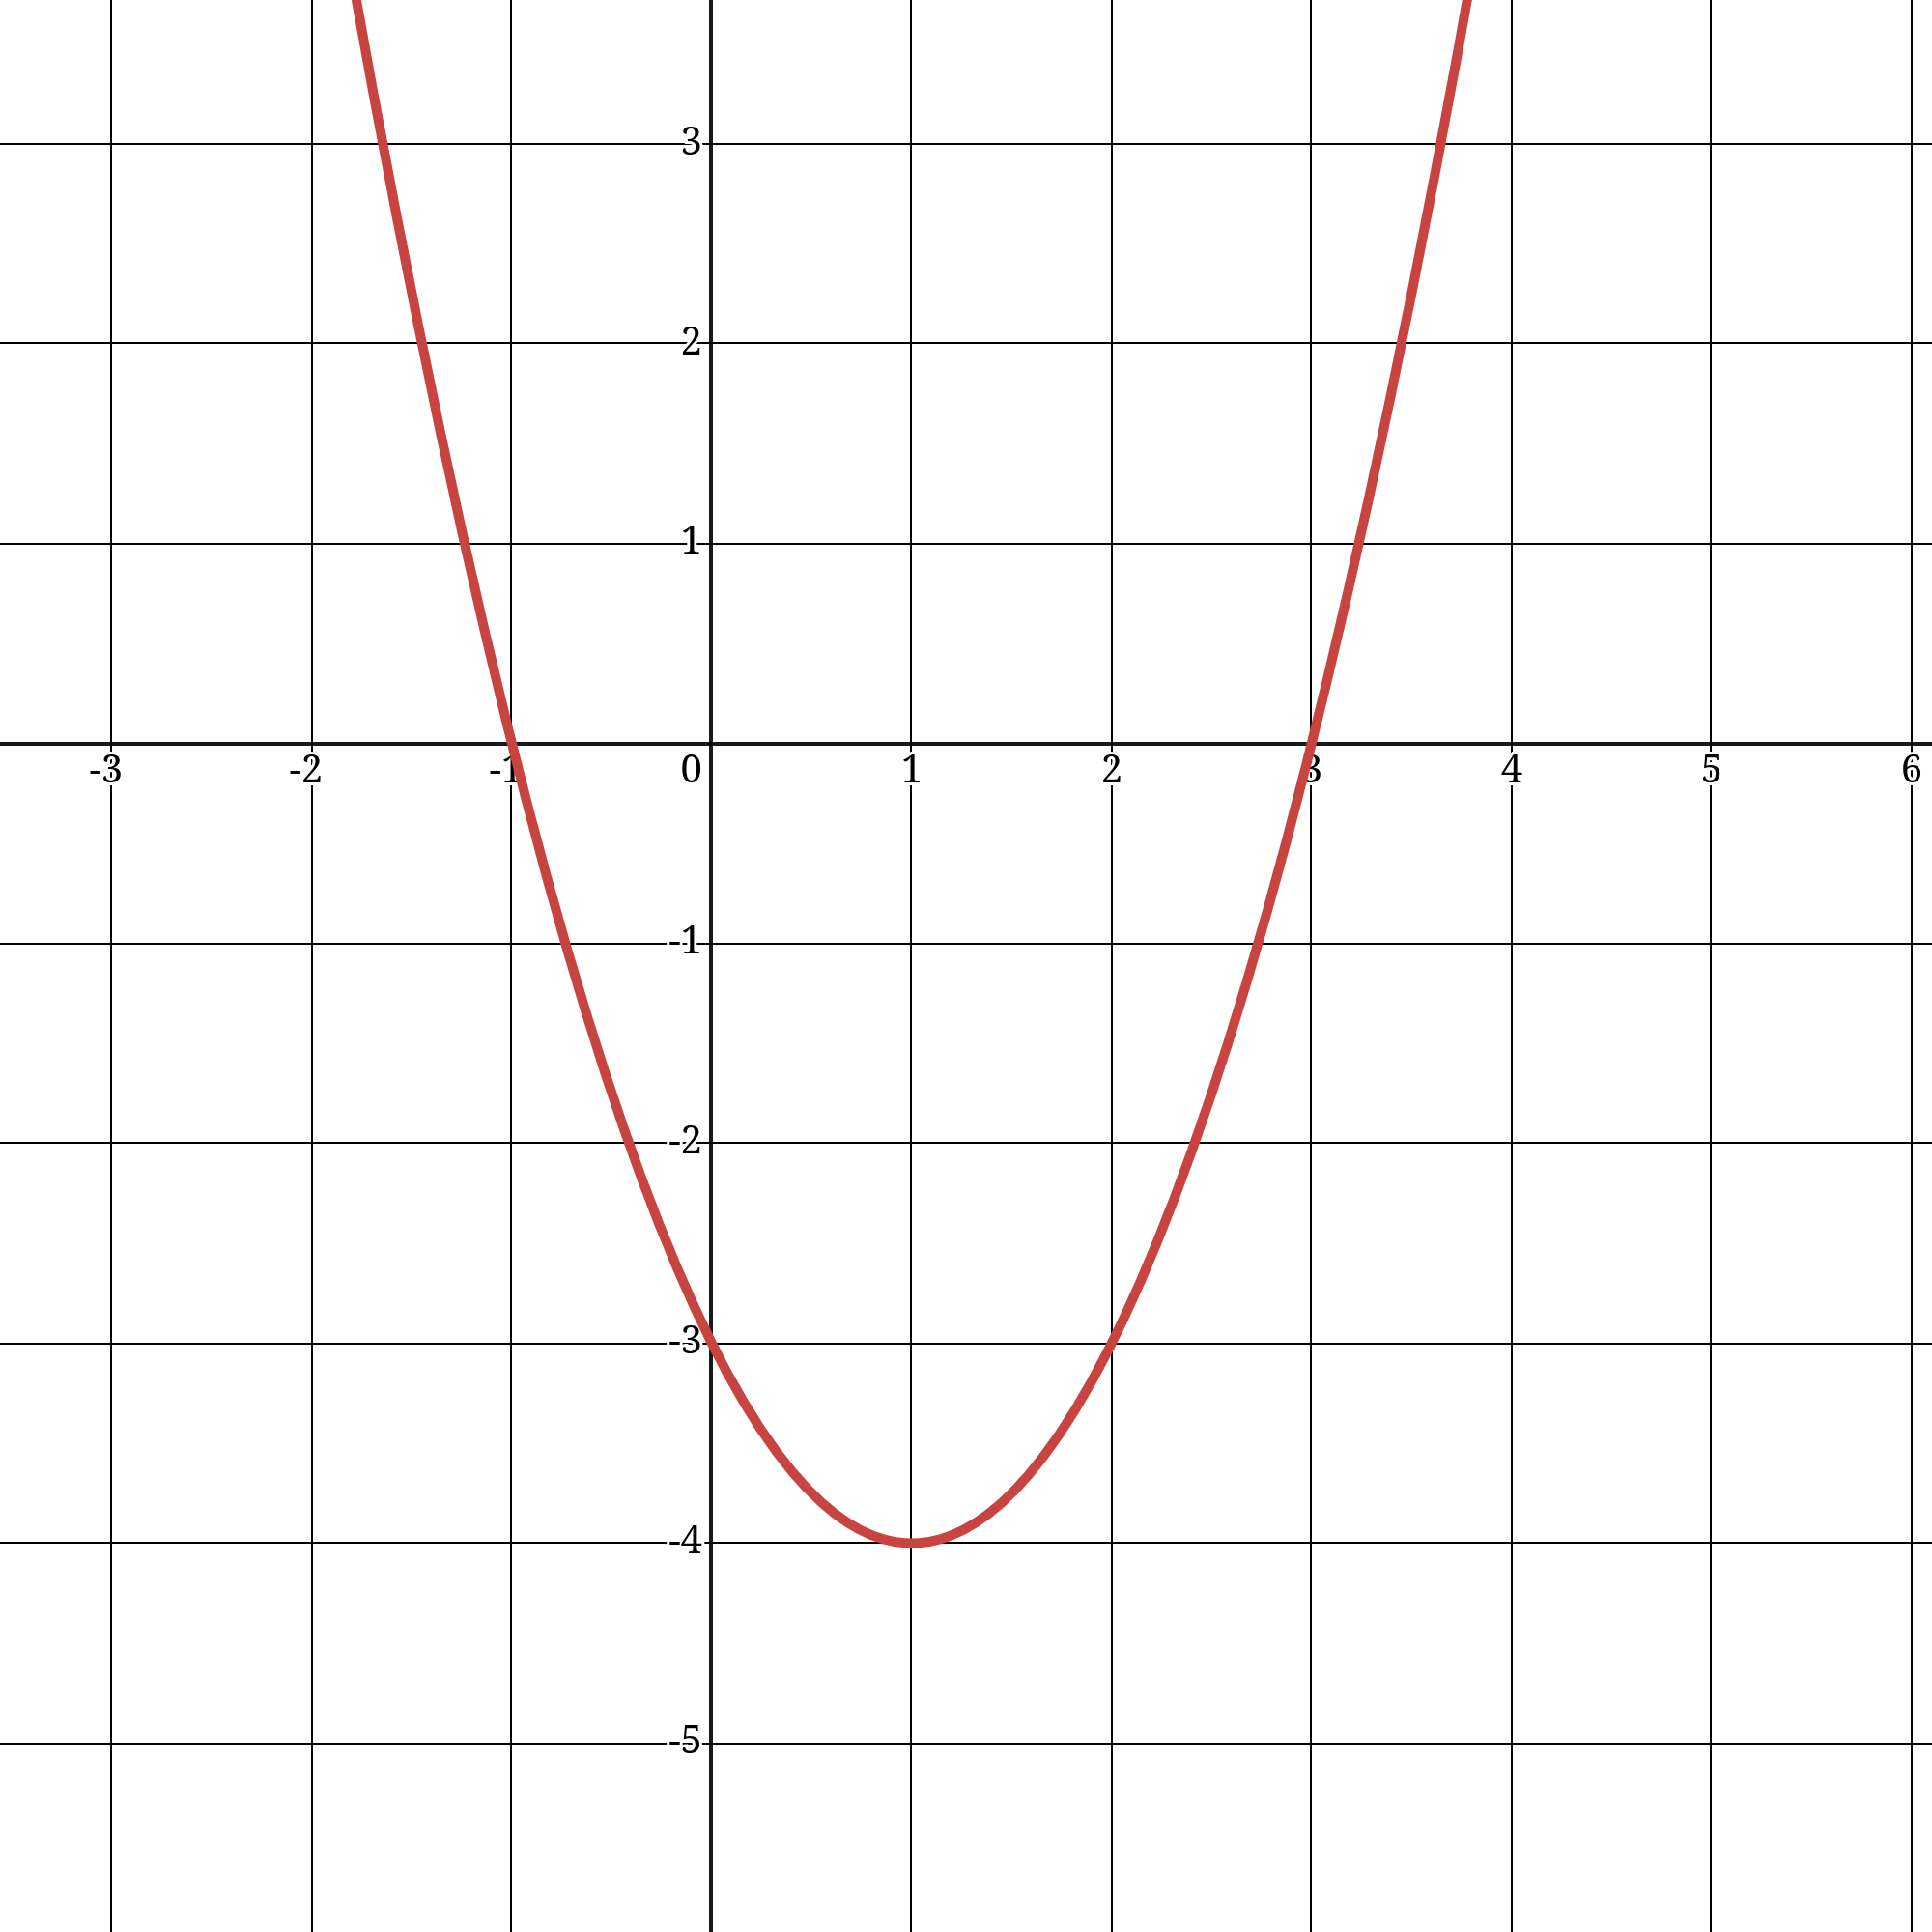
\includegraphics[scale = 0.1]{quadratic_graph}
\]

\question Evaluate the function
\[
f(x)=x^{2}+2x+3
\]
for the following function values 
\begin{enumerate}[label = \alph*)]
    \item $f(-2)=$ 
		\item $f(x+1)=$
		\item $f(-x)=$
\end{enumerate}

\question Find the relative maximum and minimums of the following graph 

\begin{figure}[htb!]
  \centering
  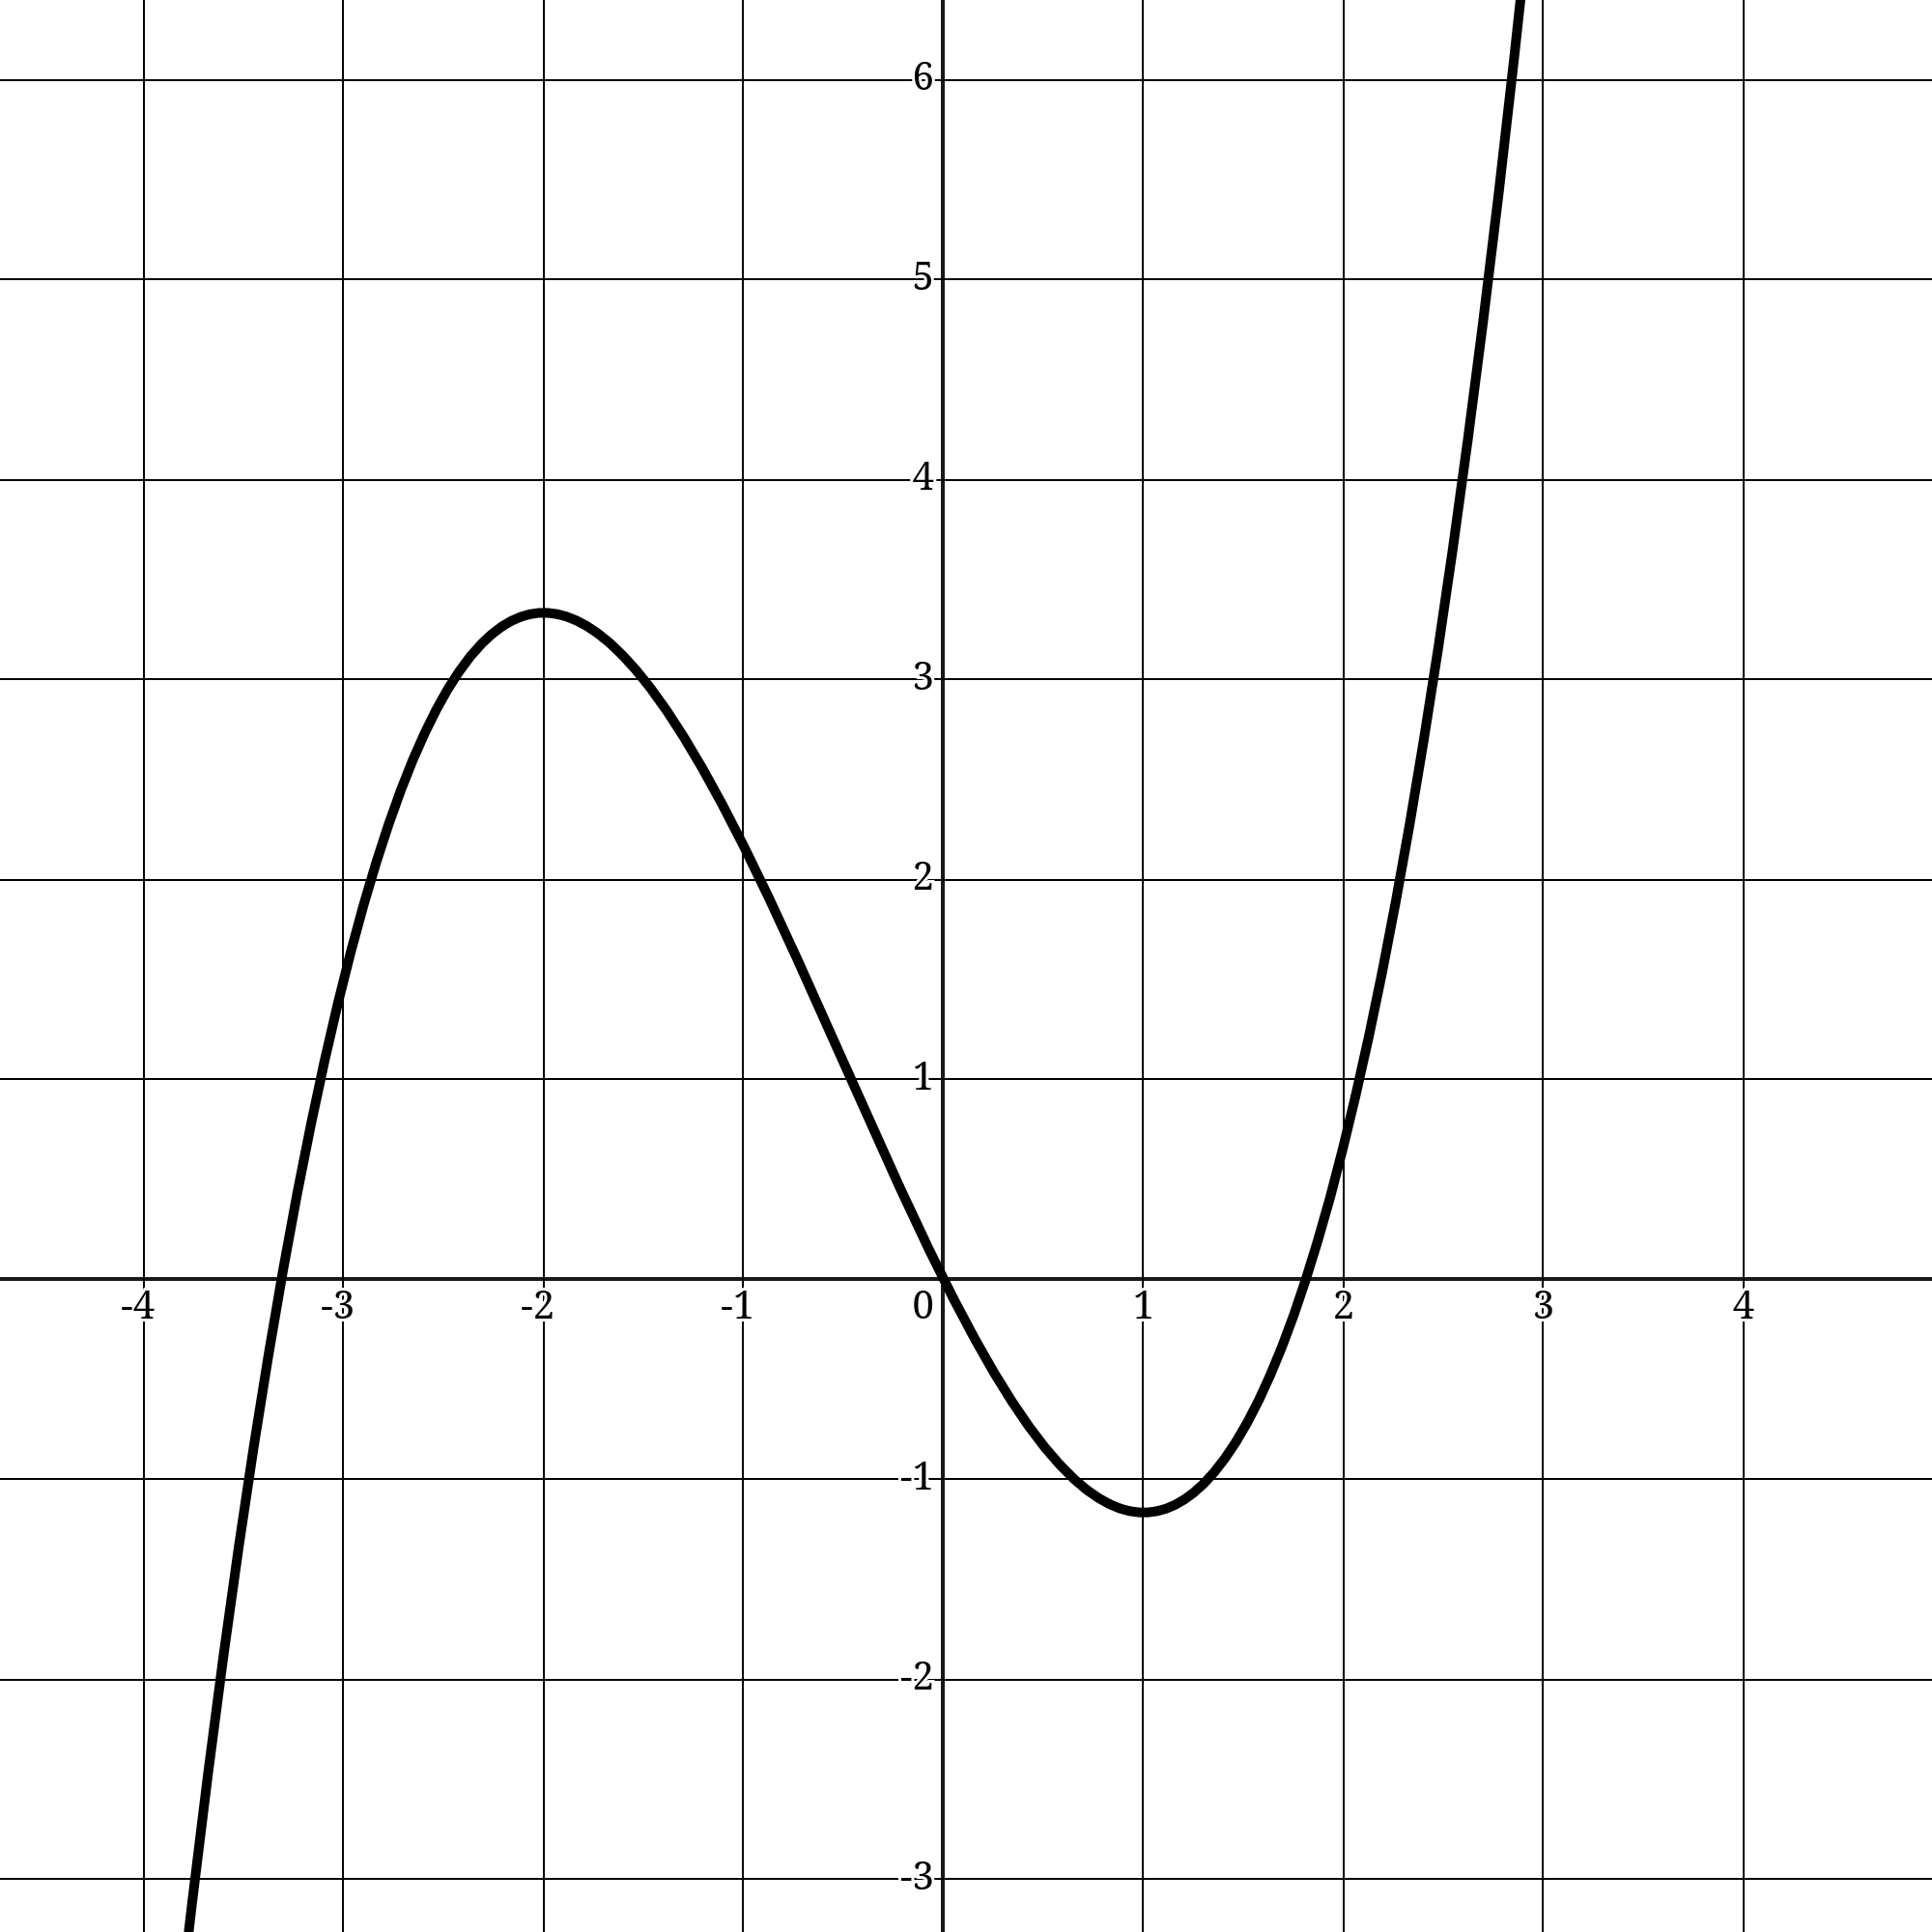
\includegraphics[scale = 0.1]{minmax}
\end{figure}

\question Give an example of an even function, and verify that it is an even function. 

\question Evaluate the following piecewise function at the following values
\[
	f(x) =
	\begin{cases}
   x+4 & x\leq -3 \\
	 -x+2 & x> -3 \\
	\end{cases}
\]

\begin{enumerate}
    \item $f(-5)=$
		\item $f(-3) = $
		\item $f(-1)= $
		\item $f(0)=$
\end{enumerate}

\end{questions}

\end{document}
